%%%%%%%%%%%%%%%%%%%%%%%%%%%%%%%%%%%%%%%%%
% Wenneker Assignment
% LaTeX Template
% Version 2.0 (12/1/2019)
%
% This template originates from:
% http://www.LaTeXTemplates.com
%
% Authors:
% Vel (vel@LaTeXTemplates.com)
% Frits Wenneker
%
% License:
% CC BY-NC-SA 3.0 (http://creativecommons.org/licenses/by-nc-sa/3.0/)
% 
%%%%%%%%%%%%%%%%%%%%%%%%%%%%%%%%%%%%%%%%%

%----------------------------------------------------------------------------------------
%	PACKAGES AND OTHER DOCUMENT CONFIGURATIONS
%----------------------------------------------------------------------------------------

\documentclass[11pt]{scrartcl} % Font size
\usepackage{algorithmic}
%%%%%%%%%%%%%%%%%%%%%%%%%%%%%%%%%%%%%%%%%
% Wenneker Assignment
% Structure Specification File
% Version 2.0 (12/1/2019)
%
% This template originates from:
% http://www.LaTeXTemplates.com
%
% Authors:
% Vel (vel@LaTeXTemplates.com)
% Frits Wenneker
%
% License:
% CC BY-NC-SA 3.0 (http://creativecommons.org/licenses/by-nc-sa/3.0/)
% 
%%%%%%%%%%%%%%%%%%%%%%%%%%%%%%%%%%%%%%%%%

%----------------------------------------------------------------------------------------
%	PACKAGES AND OTHER DOCUMENT CONFIGURATIONS
%----------------------------------------------------------------------------------------

\usepackage{amsmath, amsfonts, amsthm} % Math packages

\usepackage{listings} % Code listings, with syntax highlighting

\usepackage[english]{babel} % English language hyphenation

\usepackage{graphicx} % Required for inserting images
\graphicspath{{Figures/}{./}} % Specifies where to look for included images (trailing slash required)

\usepackage{booktabs} % Required for better horizontal rules in tables

\numberwithin{equation}{section} % Number equations within sections (i.e. 1.1, 1.2, 2.1, 2.2 instead of 1, 2, 3, 4)
\numberwithin{figure}{section} % Number figures within sections (i.e. 1.1, 1.2, 2.1, 2.2 instead of 1, 2, 3, 4)
\numberwithin{table}{section} % Number tables within sections (i.e. 1.1, 1.2, 2.1, 2.2 instead of 1, 2, 3, 4)

\setlength\parindent{0pt} % Removes all indentation from paragraphs

\usepackage{enumitem} % Required for list customisation
\setlist{noitemsep} % No spacing between list items

%----------------------------------------------------------------------------------------
%	DOCUMENT MARGINS
%----------------------------------------------------------------------------------------

\usepackage{geometry} % Required for adjusting page dimensions and margins

\geometry{
	paper=a4paper, % Paper size, change to letterpaper for US letter size
	top=2.5cm, % Top margin
	bottom=3cm, % Bottom margin
	left=3cm, % Left margin
	right=3cm, % Right margin
	headheight=0.75cm, % Header height
	footskip=1.5cm, % Space from the bottom margin to the baseline of the footer
	headsep=0.75cm, % Space from the top margin to the baseline of the header
	%showframe, % Uncomment to show how the type block is set on the page
}

%----------------------------------------------------------------------------------------
%	FONTS
%----------------------------------------------------------------------------------------

\usepackage[utf8]{inputenc} % Required for inputting international characters
\usepackage[T1]{fontenc} % Use 8-bit encoding

\usepackage{fourier} % Use the Adobe Utopia font for the document

%----------------------------------------------------------------------------------------
%	SECTION TITLES
%----------------------------------------------------------------------------------------

\usepackage{sectsty} % Allows customising section commands

\sectionfont{\vspace{6pt}\centering\normalfont\scshape} % \section{} styling
\subsectionfont{\normalfont\bfseries} % \subsection{} styling
\subsubsectionfont{\normalfont\itshape} % \subsubsection{} styling
\paragraphfont{\normalfont\scshape} % \paragraph{} styling

%----------------------------------------------------------------------------------------
%	HEADERS AND FOOTERS
%----------------------------------------------------------------------------------------

\usepackage{scrlayer-scrpage} % Required for customising headers and footers

\ohead*{} % Right header
\ihead*{} % Left header
\chead*{} % Centre header

\ofoot*{} % Right footer
\ifoot*{} % Left footer
\cfoot*{\pagemark} % Centre footer
 % Include the file specifying the document structure and custom commands
%\usepackage[demo]{graphicx}
%\usepackage{caption}
\usepackage{subcaption}
\usepackage{float}
\usepackage{listings}
\usepackage[showframe=true]{geometry}
\usepackage{changepage}

%----------------------------------------------------------------------------------------
%	TITLE SECTION
%----------------------------------------------------------------------------------------

\title{	
	\normalfont\normalsize
	\textsc{Università degli Studi di Trieste}\\ % Your university, school and/or department name(s)
	\vspace{25pt} % Whitespace
	\rule{\linewidth}{0.5pt}\\ % Thin top horizontal rule
	\vspace{20pt} % Whitespace
	{\huge First FHPC Assignment}\\ % The assignment title
	\vspace{12pt} % Whitespace
	\rule{\linewidth}{2pt}\\ % Thick bottom horizontal rule
	\vspace{12pt} % Whitespace
}

\author{\LARGE Nicola Domenis} % Your name

\date{\normalsize\today} % Today's date (\today) or a custom date

\begin{document}

\maketitle % Print the title

%----------------------------------------------------------------------------------------
%	FIGURE EXAMPLE
%----------------------------------------------------------------------------------------

\section{Preview}
 
In this assignment we will present the following subjects:

\begin{itemize}
	\item the production of a parallel program code
	\item the graphs of the theoretical and real speedup of the code
	\item anything else
\end{itemize}


%------------------------------------------------
\section{section 0}
\subsection{Laptop theoretical peak performance}

We want to calculate the theoretical peak performance of our own portable computer by using the formula \textit{theoretical peak performance} = clock frequency x FLOPs x number of cores.
We gather that \textit{clock frequency} $= 2.90 Ghz$,$ FLOPs = 16$ and $numberofcores = 2$ for our computer architecture,an intel i7 with a Kaby Lake microarchitecture; thus we compute \textit{theoretical peak performance} $= 92.8 GFlops/s$
%Vect_size = dimensione di registro vettoriale stessa operaaxione nello stesso momento diviso dimensione double:andiamo a vedere se ci sono le sigle (mmx sse)128bit 2 double (avx avx2) 256bit 4 double (avx512)512bit 8 double
%primo fattore
%
%cercare FMA fused multiply addiction A = BxC+D  vec
%vector_size*2*#fma

%quanti cicli ci vogliono? pensiamo che sia 1 = 1*vector_size*2*#fma

%numero di operazioni in double precision
%\begin{figure}
%\begin{adjustwidth}{-2cm}{}
\begin{table}[H]
		\begin{tabular}[H]{l| l| l| l| l| l }
			&Your model&CPU&Frequency&Number of Cores&Peak Performance\\
			laptop& Asus F556U & Intel Core i7-7500 &$2.90$ GHz&2&92.8 GFLOPs/s
		\end{tabular}
	\label{Result}
\end{table}
%\end{adjustwidth}
%\end{figure}

\subsection{Smartphone theoretical peak performance}
We installed "`Mobile Linpack"' app and we run a few test. We report here some results,even on repeated trials: 
%\begin{figure}
\begin{adjustwidth}{-2cm}{}
	\begin{tabular}[H]{l| p{0.2\textwidth}| l |l| l|l }
		\hline
			&Model& Sustained performance&Matrix size&Peak performance&Memory\\
			\hline
			Cellphone&Samsung Galaxy XCover 4 &114,81 Mflops/s &250 &not calculated&16,00 GB\\
			& &145.53 Mflop/s&500& &\\
			& &157.5 Mflop/s&800& &\\
			& &201.32 Mflop/s&800& &\\
			& &155.93 Mflop/s&900& &\\
			& &109.88 Mflop/s&1000& &\\
			& &103.14 Mflop/s&2000& &\\
		\end{tabular}
\end{adjustwidth}
%\end{figure}

\subsection{Laptops,smartphones and the top 500}
Let's check now whether our technologies would have competed with the Top500 supercomputers in the past:
%\begin{figure}
\begin{adjustwidth}{-2cm}{}
	\begin{tabular}[H]{p{0.15\textwidth}| p{0.15\textwidth}| p{0.15\textwidth} | p{0.3\textwidth}| p{0.3\textwidth}}
		\hline
			&Model&Performance&Top 500 year\& position&number 1 HPC system\\
			\hline
			Smartphone&Samsung Galaxy XCover 4 &201,32 Mflops/s &does not enter in the top500 of the first year of measurement, the 500th Supercomputer has an Rmax of 0.5 GFlops/s (equal to 2.4 times our smartphone peak performance)& Numerical Wind Tunnel,Fujitsu National Aerospace Laboratory of Japan is first in the year 1993 with a Rmax equal to 124.0 GFlops/s (equal to 616 times our cellphone's sustained peak performance)\\
			\hline
			Laptop&ASUS F556U&92.8 GFLOPs/s& 3rd position at nov 1993. Remains in the top 10 until nov 1996 & We have the same top position with a Rpeak equal to 235.8 GFlops/s(equal to 2.5 times our laptop's theoretical peak performance)\\
		\end{tabular}
\end{adjustwidth}
%\end{figure}

%\begin{table}
	%\centering
		%\begin{tabular}{l| l| l |l| l| l}
			%&Model& Sustained performance&Matrix size&Peak performance&Memory\\
			%Cellphone&Samsung Galaxy XCover 4 &114,81 Mflops/s &250 &not calculated&16,00 GB
			%&&145.53 Mflop/s&500&&
			%&&157.5 Mflop/s&800&&
			%&&109.88 Mflop/s&1000&&
		%\end{tabular}
	%\label{Quick test parameters and results}
%\end{table}

%----------------------------------------------------------------------------------------
%	TEXT EXAMPLE
%----------------------------------------------------------------------------------------

\section{Section 1}

\subsection{Model for a serial and parallel summation of n numbers}
Here we discuss about modeling a simple program which consists of summing n numbers.
A simple pseudocode for the serial program would be:


\begin{algorithmic}

\STATE {Data:array $A[]$ of values}
\FOR{i from 1 to n} \STATE {sum = sum + A[i]} \ENDFOR
\RETURN{sum}
\end{algorithmic}

If we choose $T_{comp}$ as the time to compute a floating point operation we could calculate the total time of a serial computation as
$T_s = N * T_{comp}$,whereas the code simply computes N times(the size of the problem) the sum of two values.

For the parallel program we complicate a little the execution:

\begin{algorithmic}

\STATE {Data:array $A[]$ of values}
\STATE {Environment: p parallel processors}
\IF {Master process}

		\STATE{Read and Split $A[]$ into p subarrays $A_i[]$}
		\STATE{Send $p-1$ subarrays to the other $p-1$ processors}
		\FOR{i from $1$ to n/p} \STATE {$sum_0 = sum_0 + A_0[i]$} \ENDFOR
		\STATE{Collect the resulting $p-1$ values $sum_i$ from the processors}
		\FOR{i from $1$ to p} \STATE {$sum = sum + sum_i$} \ENDFOR
\ENDIF
\IF {Slave process}
	\STATE{Receive subarrays $A_i[]$ from the Master process}
	\FOR{i from 1 to n/p} \STATE {$sum_i = sum_i + A_i[i]$} \ENDFOR
	\STATE{Send $sum_i$ back to the Master process}
\ENDIF
\RETURN{sum}
\end{algorithmic}

If we define the times $T_{read}$ to indicate the time needed to read a variable,and $T_{comm}$ to indicate the time needed to communicate a variable, we can deduce the theoretical execution time of the model:
\  
\begin{algorithmic}
		\STATE{Read and Split $A[]$ into p subarrays $A_i[]$}
		\STATE{EXECUTION TIME: $T_{read}$}
\end{algorithmic}
\ 
\begin{algorithmic}
		\STATE{Send $p-1$ subarrays to the other $p-1$ processors}
		\STATE{EXECUTION TIME: $T_{comm}*(p-1)$}
\end{algorithmic}
\ 

\begin{algorithmic}

\FOR{i from $1$ to $n/p$} \STATE {$sum_i = sum_i + A_i[i]$} \ENDFOR
\STATE{EXECUTION TIME: $n/p * T_{comp}$}
\STATE{This is a parallel execution, the subarrays are added inside each processor}	
\end{algorithmic}

\ 
\begin{algorithmic}
\STATE{Send $sum_i$ back to the Master process}
\STATE{EXECUTION TIME: $(p-1)*T_{comm}$}
\end{algorithmic}
\ 
\begin{algorithmic}
		\FOR{i from $1$ to p} \STATE {$sum = sum + sum_i$} \ENDFOR
		\STATE{EXECUTION TIME: $(p-1)*T_{comp}$}
\end{algorithmic}

The total sum of the execution times gives $T_p = T_{read} + (p-1+n/p)*T_{comp}+2*T_{comm}(p-1)$. We can calculate it with the theoretical values $T_{comp} =2 \times 10^{-9}$,$T_{read}= 1 \times 10^{-4}$ and $T_{comm}= 1 \times 10^{-6}$
%----------------------------------------------

\subsection{Scalability of the Model}

Once we have the theoretical $T_p$ and $T_s$ we can calculate the Speedup given by the formula $Speedup(p)=T_s/T_p$ . We give the following plots on the variable $p$:

%\begin{figure}
%\centering
%\begin{subfigure}{.5\textwidth}
	%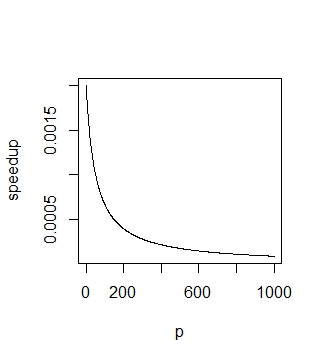
\includegraphics[width=0.5\columnwidth]{Rplot_speedup_4} % Example image
	%\caption{Speedup for $N=10^2$,maximum: $speedup = 0.00199$ at $p = 1$}
%\end{subfigure}%
%\begin{subfigure}{.5\textwidth}
 %% [h] forces the figure to be output where it is defined in the code (it suppresses floating)
	%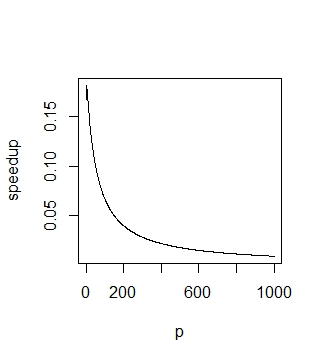
\includegraphics[width=0.5\columnwidth]{Rplot_speedup_3} % Example image
	%\caption{Speedup for $N=10^4$,maximum: $speedup = 0.180$ at $p = 3$}
 %\end{subfigure}
%\end{figure}

\begin{figure}[H] % [h] forces the figure to be output where it is defined in the code (it suppresses floating)
	\centering
	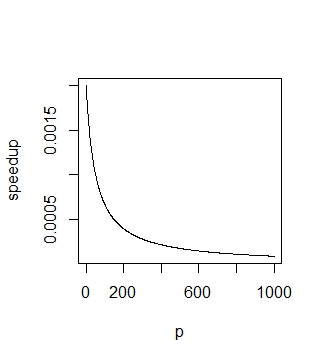
\includegraphics[width=0.6\columnwidth]{Rplot_speedup_4} % Example image
	\caption{Speedup for $N=10^2$,maximum: $speedup = 0.00199$ at $p = 1$}
\end{figure}


\begin{figure}[H] % [h] forces the figure to be output where it is defined in the code (it suppresses floating)
	\centering
	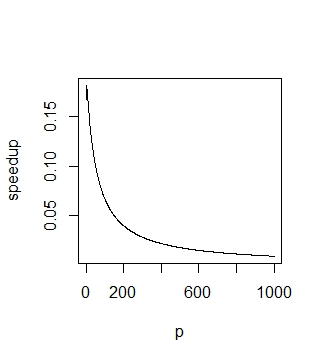
\includegraphics[width=0.6\columnwidth]{Rplot_speedup_3} % Example image
	\caption{Speedup for $N=10^4$,maximum: $speedup = 0.180$ at $p = 3$}
\end{figure}

%\begin{figure}
%\centering
%\begin{subfigure}{.5\textwidth}
 %% [h] forces the figure to be output where it is defined in the code (it suppresses floating)
	%\centering  %
	%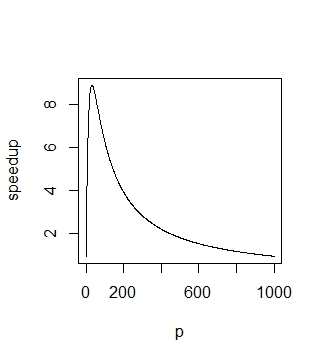
\includegraphics[width=0.6\columnwidth]{Rplot_speedup_!} % Example image
	%\caption{Speedup for $N=10^6$,
	%maximum: $speedup = 8.90$ at $p = 32$}
%\end{subfigure}%
%\begin{subfigure}{.5\textwidth}
%\centering
%% [h] forces the figure to be output where it is defined in the code (it suppresses floating)
	%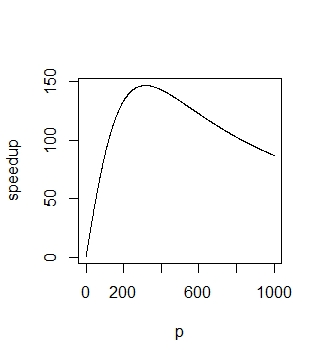
\includegraphics[width=0.6\columnwidth]{Rplot_speedup_2} % Example image
	%\caption{Speedup for $N=10^8$,
	%maximum: $speedup = 146.67$ at $p = 316$}
 %\end{subfigure}
%\end{figure}
\begin{figure}[H] % [h] forces the figure to be output where it is defined in the code (it suppresses floating)
	\centering
	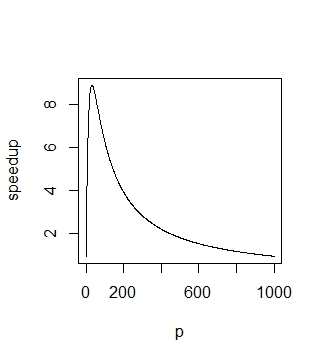
\includegraphics[width=0.6\columnwidth]{Rplot_speedup_!} % Example image
	\caption{Speedup for $N=10^6$,maximum: $speedup = 8.90$ at $p = 32$}
\end{figure}
\begin{figure}[H] % [h] forces the figure to be output where it is defined in the code (it suppresses floating)
	\centering
	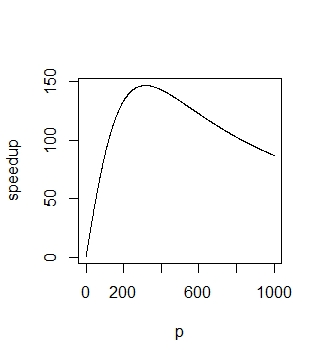
\includegraphics[width=0.6\columnwidth]{Rplot_speedup_2} % Example image
	\caption{Speedup for $N=10^8$,maximum: $speedup = 146.67$ at $p = 316$}
\end{figure}

We notice that this is a case of strong scaling, where adding a certain number of processors accelerate the calculations of a same-size problem, but only to a certain point. After the maximum, the communication time overpowers the advantage of the parallelization, thus lowering the speedup. Simply adding processors to the calculus will not speed up the process because the time it takes to the master node to assign the subarray to the slaves will become too high to be easily computed.
This is different when we have a high problem size, starting from around $N=10^4$
we see that the model starts scaling from p=1 to the maximum of the plot.
%------------------------------------------------
\section{Section 2}

\subsection{mpi\_pi.c and pi.c execution}
We start by executing the two codes pi.c and mpi\_pi.c we have:

\begin{lstlisting}[language=bash]
  
$ g++ pi.c -o pi.x
$ time ./pi.x 10000000

 # of trials = 10000000 , estimate of pi is 3.141396400 

 # walltime : 0.19000000 

real    0m0.275s
user    0m0.271s
sys     0m0.001s
\end{lstlisting}
And the parallel file:
\begin{lstlisting}[language=bash]
$ mpicc mpi_pi.c -o mpi_pi.x
$ time mpirun -np 10 ./mpi_p.x 10000000

 # walltime on processor 1 : 0.02612305 

 # walltime on processor 2 : 0.03022003 

 # walltime on processor 3 : 0.02638388 

 # walltime on processor 4 : 0.03122497 

 # walltime on processor 5 : 0.02647901 

 # walltime on processor 6 : 0.02861810 

 # walltime on processor 7 : 0.03266811 

 # walltime on processor 8 : 0.02701306 

 # walltime on processor 9 : 0.03131413 

 # of trials = 10000000 , estimate of pi is 3.141720800 

 # walltime on master processor : 0.06575489 

real    0m1.890s
user    0m11.881s
sys     0m0.630s
\end{lstlisting}

We should get the longest time of all the parallel execution times of mpi\_pi.x in order to asses its speed.

Let's collect various run times for a different number of processors.
%------------------------------------------------
\begin{adjustwidth}{2cm}{}
	\begin{tabular}[h]{l|l }
		\hline
			\# of processors&Master processor speed\\
			\hline
			1&0.19828200\\
			2&0.10205293\\
			4&0.05147886\\
			8&0.04555607\\
			16&0.01546288\\
			32&0.00758505\\
		\end{tabular}
	\end{adjustwidth}
We notice that the serial run time above and the 1-processor parallel run time on this table differ because of the parallel overhead time: $T_p(1)-T_s= 0.19828-0.190000 = 8.28 ms$
Those values are plotted as:
\begin{figure}[H] % [h] forces the figure to be output where it is defined in the code (it suppresses floating)
	\centering
	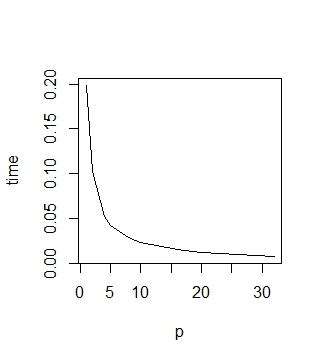
\includegraphics[width=0.6\columnwidth]{Rplot_speed_p2} % Example image
	\caption{Speed vs number of processors graph}
\end{figure}

The time decreases with an inverse proprotionality to the time. Now lets plot the speedup: 
\begin{figure}[H] % [h] forces the figure to be output where it is defined in the code (it suppresses floating)
	\centering
	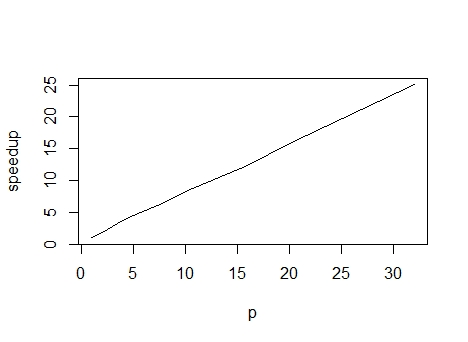
\includegraphics[width=0.6\columnwidth]{Rplot_speedup_pi} % Example image
	\caption{Speedup vs number of processors graph}
\end{figure}
We see that it is linear,thus we have strong scalability: as we increase the number of processors we obtain a faster parallel program.

Let's repeat our observations by having a larger number of parallel processors.
Here we have a plot that shows us the master execution time according to the number of processors. The times are not strictly decreasing because the processor is less scalable as p grows. Lets see the case N=10^7
\begin{figure}[H] % [h] forces the figure to be output where it is defined in the code (it suppresses floating)
	\centering
	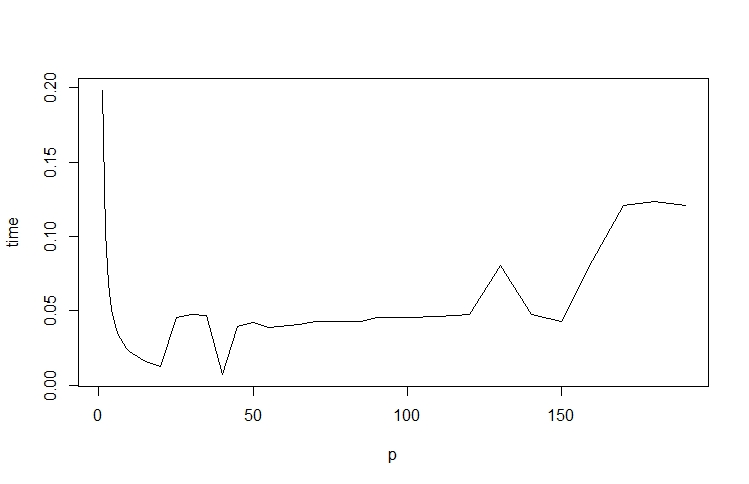
\includegraphics[width=0.6\columnwidth]{Rplot_pi_master_execution} % Example image
	\caption{N= 10^7Execution time vs number of processors}
\end{figure}
We can see that the speedup  decreases for a large number of processors
\begin{figure}[H] % [h] forces the figure to be output where it is defined in the code (it suppresses floating)
	\centering
	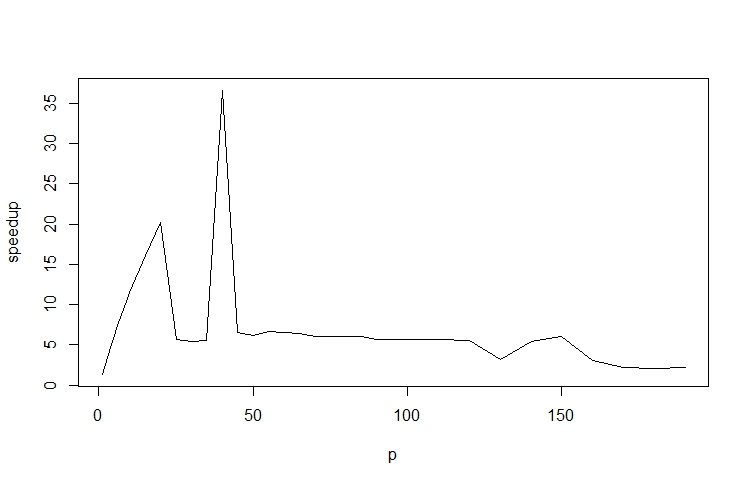
\includegraphics[width=0.6\columnwidth]{Rplot_pi_speedup_many_processors} % Example image
	\caption{N=10^7Speedup vs number of processors}
\end{figure}
We can observe the first linear growth that we plotted earlier. The speedup then decreases.
Lets see the same graphs for N=10^8:
\begin{figure}[H] % [h] forces the figure to be output where it is defined in the code (it suppresses floating)
	\centering
	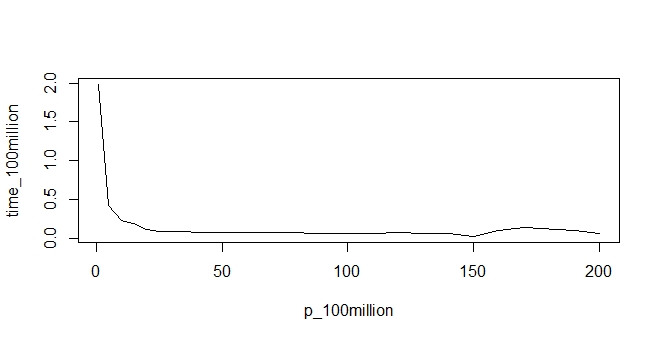
\includegraphics[width=0.6\columnwidth]{Rplot_pi_as_100million_time} % Example image
	\caption{N= 10^8 execution time vs number of processors}
\end{figure}
\begin{figure}[H] % [h] forces the figure to be output where it is defined in the code (it suppresses floating)
	\centering
	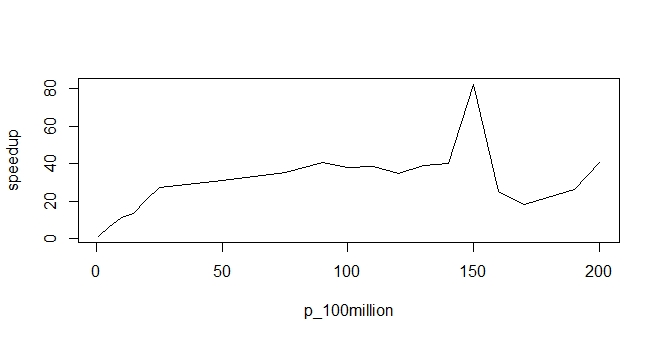
\includegraphics[width=0.6\columnwidth]{Rplot_pi_as_100millions_speedup} % Example image
	\caption{N= 10^8 speedup vs number of processors}
\end{figure}
Now lets see the results for N=10^9:
\begin{figure}[H] % [h] forces the figure to be output where it is defined in the code (it suppresses floating)
	\centering
	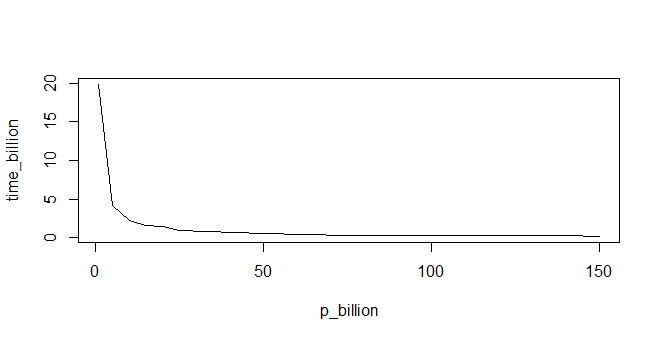
\includegraphics[width=0.6\columnwidth]{Rplot_pi_as_billions} % Example image
	\caption{N= N=10^9 execution time vs number of processors}
\end{figure}
\begin{figure}[H] % [h] forces the figure to be output where it is defined in the code (it suppresses floating)
	\centering
	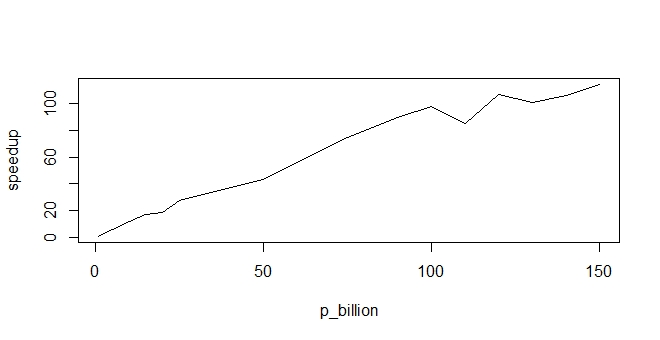
\includegraphics[width=0.6\columnwidth]{Rplot_pi_as_billions_speedup} % Example image
	\caption{N= N=10^9 speedup vs number of processors}
\end{figure}

Here the plot is much clearer
 We have modeled the strong scalability of the program
%----------------------------------------------------------------------------------------
%	EQUATION EXAMPLES
%----------------------------------------------------------------------------------------

\section{Section 3}


\subsection{The written code}
Now we will focus on the two codes that represent an implementation of the theoretical model for the summation of the first n integers. We have the serial implementation in the code \textsc{sum\_of\_n.c} and the parallel implementation of the code \textsc{sumNumbers\_mpi.c}.
Let's try the code for $n=1000$:
\begin{lstlisting}[language=bash]
$ g++ sum_of_n.c -o sum_of_n.x
$ time ./sum_of_n.x < n.txt
total sum: 500500
real    0m0.005s
user    0m0.000s
sys     0m0.002s

$ module load openmpi
$ mpicc mpi_sum_of_n.c -o mpi_sum_of_n.x -std=c11
time mpirun -np 10 ./mpi_sum_of_n.x < n.txt
time spent on process 1 is 0.000041 seconds
time spent on process 2 is 0.004197 seconds
time spent on process 3 is 0.000022 seconds
time spent on process 4 is 0.009296 seconds
time spent on process 5 is 0.004883 seconds
time spent on process 6 is 0.000022 seconds
time spent on process 7 is 0.008823 seconds
total sum: 500500 
time spent on process 0 is 0.023464 seconds
time spent on process 8 is 0.000022 seconds
time spent on process 9 is 0.004411 seconds

real    0m1.853s
user    0m11.561s
sys     0m0.635s
\end{lstlisting}

Let's try again with N=1000000000 and p = 10. We collect a few particular times of the execution:

\begin{align} 
	\begin{split}
		T_{read}&= 3.38554 e-05 seconds\\
		T_comp (N/P)&= 0.355836\\
		\rightarrow T_{comp} = 0.355836/100000000 = 3.5836e-9
		T_comm&=2.14577e-06
	\end{split}					
\end{align}
 We see that those values are close to the theoretical values we gave before
%------------------------------------------------



%----------------------------------------------------------------------------------------
%	LIST EXAMPLES
%------------------------------------------------------------------------------


%----------------------------------------------------------------------------------------

%-------------------------------------------------------------

%------------------------------------------------

%----------------------------------------------------------------------------------------

\end{document}
